\chapter{REVIEW OF RELATED LITERATURE}
{\baselineskip=2\baselineskip
This literature review explores current weight estimation techniques in livestock management, highlighting the advancements and limitations of traditional methods while introducing emerging technologies, particularly depth-sensing devices like the Kinect sensor. Understanding the shift from conventional approaches to tech-driven solutions provides insight into how these innovations can improve accuracy, efficiency, and scalability in livestock farming.

%-----------------------------------------------------------------------------------------------------------------------
\section{Weight Estimation Techniques}
In animal production, livestock body weight is a significant and widely used feature that has an impact on feed consumption, breeding potential, social behavior, energy balance, and overall farm management \citep{wang2024review}. It may be used indirectly in the assessment of health and welfare status \citep{dikmen2012effect}. There are two main approaches to measuring body weight in livestock: (1) direct approaches using scales, and (2) indirect approaches based on relationships between body part measurement and body weight.

Direct weighing methods rely on weighing technologies such as partial-weight or full-weight industrial scales capable of supporting small, medium, or large livestock. Some companies provide passive-weighing solutions that integrate sensor-rich scaling systems such as GrowSafe of Canada, the Bosch Precision Livestock Platform of Germany, and Rice Lake Weighing Systems of Australia which are capable to measure, log results, and transmitting information over wired or wireless networks \citep{wang2024review} . Other companies such as Arvet CIMA Control Pig and CIMA Control Cow Scaling Systems of Spain developed custom-made scales that provide dynamic-weighing systems where animals are weighed while in motion using walk-through or step-over weighers \citep{rousing2004stepping}. While these devices are very accurate, their acquisition, intended purpose and operation size, repeated calibration and maintenance costs associated with their placement in high-temperature variability, and corrosive environments are significant and beyond the affordability and sustainability limits of small and medium size farms and even commercial operators\citep{dikmen2012effect}. It has been studied that removing animals from paddocks and holding areas and leading them to weighing stations is costly, stressful, and potentially harmful activity for animals and handlers alike and also inadvertently leads to animal weight loss or even death \citep{faucitano2018transport}. Moreover, since the weighing process is very laborious, the frequency of measurements is not sufficiently high to permit the use of body weight as an indicator for other traits. However, since the affordability of direct weighing methods may impede small producers \citep{dickinson2013automated}, researchers have developed indirect weighing methods represented by regression models that relate morphometric measurements and image features to body weight in livestock. The direct acquisition of morphometric measurements can be accomplished with the aid of technologies with various degrees of complexity, from measuring tapes and types to specialized software or manual, semi-automatic, or automatic measurements extrapolated from images obtained with electro-optical devices such as mono-2D, stereo-2D, 3D, ultrasound, and infrared sensors \citep{wang2024review}.

\subsection{Role of Technology in Agriculture}

Technological advancements have played a pivotal role in transforming the agricultural sector. From mechanization to digital innovations, these technologies have increased efficiency, productivity, and sustainability in farming practices. In particular, precision agriculture, which uses technology to optimize field-level management of crop farming, has revolutionized the way food is produced \citep{witten1993practical}. Precision farming technologies include GPS, soil sensors, and drones, allowing farmers to monitor and manage their crops with unprecedented accuracy.
In livestock farming, technology has led to the development of automated feeding systems, health monitoring tools, and weight estimation systems that reduce labor and enhance animal welfare \citep{gomez2021systematic}. For example, sensor-based systems for monitoring livestock health provide farmers with real-time data, enabling proactive interventions to prevent diseases and improve overall herd management \citep{neethirajan2021digital}.

Furthermore, AI and machine learning have started to play an increasingly significant role in agriculture. These technologies enable predictive analytics for crop yields and disease outbreaks, and more recently, they are being used in 3D object detection systems for animal weight estimation, such as the Kinect-based system for pig weight estimation proposed in this study \citep{farooqui2024precision}. Integrating AI and machine learning into agricultural practices is expected to address many challenges related to food security, sustainability, and labor shortages \citep{ng2023machine}.

For example, one study explored the use of 3D images captured from a zenithal viewpoint to estimate lambs' live weight. The researchers applied image processing techniques to extract features such as upper body area and average depth, demonstrating the potential of 3D imaging for livestock weight estimation \citep{samperio2021lambs}. Although this study did not use Kinect, it highlights the value of 3D data, which Kinect is well-equipped to provide, for accurate livestock weight estimation.

Another significant study used the Microsoft Kinect V1 depth camera to measure pig body dimensions and estimate their weight. The researchers found a strong correlation between the Kinect-based measurements and actual weights, with coefficients of determination (R²) exceeding 0.90 \citep{pezzuolo2018barn}. Similarly, Lao et al. also employed a Kinect V1 depth camera to extract body measurements from pigs, developing a regression model for weight estimation, while Liu et al. used a binocular vision system to collect 3D data and tested various modeling approaches, including linear, nonlinear, and machine learning algorithms, to estimate pig weight \citep{li2014estimation}.


\section{Technological Frameworks}

The manual techniques used in the majority of livestock weight estimation systems today have given way to more automated, technologically advanced systems. Physical weighing scales, which were labor-intensive, time-consuming, and frequently uncomfortable for animals, were the foundation of traditional methods. On the other hand, cutting-edge image technologies are now used in modern systems, including 3D depth sensors like the Microsoft Kinect and binocular and monocular vision systems. For extremely precise 3D reconstructions of animals, binocular vision systems employ two cameras to collect stereo images; however, the expense and complexity of these installations may make them impractical for small farms \citep{rousing2004stepping}. Compared to binocular vision systems, monocular vision systems, which use single-camera setups, are more affordable but have worse precision.

Smart sensors are at the vanguard of revolutionizing precision agriculture by giving farmers access to real-time information on vital parameters including plant health, temperature, humidity, and soil moisture. With their sophisticated detection methods, these sensors assist farmers in making well-informed decisions that increase crop output. Farmers may automate and optimize tasks like nutrient application and irrigation scheduling by combining these sensors with Internet of Things (IoT) devices and artificial intelligence (AI). By giving real-time data on vital elements like soil moisture, temperature, humidity, and plant health, smart sensors are transforming precision agriculture. Farmers can better control fertilizers, optimize irrigation, and monitor crop conditions by integrating these sensors with IoT and AI technologies. This contributes to resource conservation, increased crop yields, and addressing environmental issues \citep{soussi2024smart}. In general, smart sensors assist in addressing issues related to global agriculture, including depletion of resources, climate change, and rising food production demands.

In general, smart sensors help address problems associated with global agriculture, such as resource depletion, climate change, and increased need for food production. Furthermore, these sensors have started to become extremely important in cattle farming. For example, smart sensors assist farmers in ensuring the comfort and welfare of their livestock by keeping an eye on environmental factors like temperature and air quality in animal housing. Thus, healthier animals and lower veterinary expenses can be achieved by preventing heat stress and disease outbreaks\citep{terence2024systematic}.

The physical characteristics of cattle, such as weight and body dimensions, can be monitored non-invasively using Computer Vision (CV)-Based Sensors, which are frequently combined with AI algorithms. Since no direct contact is required, methods like RGB picture analysis and 3D point cloud offer great accuracy and can lessen animal suffering \citep{ma2024computer}. These technologies have the potential to greatly increase the accuracy of data gathered for monitoring, enabling better cattle care and management. However, small-scale farms face difficulties due to the complexity of establishing computer vision systems, which sometimes require pricey hardware and intricate data processing \citep{terence2024systematic}.  High initial investments are needed for computer vision systems, especially those that use 3D cameras and intricate algorithms. Particularly for smaller farms, the expense of high-quality technology (such as RGB cameras or 3D scanners) and the required computer infrastructure can be prohibitive. 

CV-based systems not only provide budgetary difficulties but also demand specialized staff to properly run and maintain the technology. Farmers may find it difficult to handle system calibrations and solve problems if they lack technical skills. This could lead to erroneous data collecting and less-than-ideal herd management results. Furthermore, the accuracy of the system may be reduced in real-world situations due to environmental conditions like dust, lighting, or even the movement of the animals that impair sensor performance \citep{ma2024computer}. Research is being done to make these technologies more resilient and affordable as they develop, so smaller operations can use them. Nonetheless, these technologies have a great deal of promise to improve livestock monitoring by lowering stress and increasing management effectiveness, even in the face of obstacles.

\section{Image Processing and Machine Learning for Weight Estimation}

\subsection{Historical Development}

In traditional livestock management, weight estimation was primarily performed manually using techniques such as Body Condition Scoring (BCS). This method evaluates the fatness or thinness of animals through visual inspection and tactile assessment \citep{bercovich2013development}. While straightforward and cost-effective, BCS relies heavily on the evaluator's expertise, introducing variability and potential bias in results. Additionally, this method does not provide precise numerical weight values, making it less reliable for data-driven decision-making in modern farming practices.

Before the introduction of digital technologies, farmers used scales or manual measurements to estimate livestock weight. With scales, animals were weighed directly, but this required significant infrastructure, such as livestock-specific weighing platforms. These setups were costly, labor-intensive, and often stressful for the animals, impacting their health and productivity.

For situations where scales were unavailable, farmers traditionally estimated pig weight using a tape measure and mathematical formulas. This approach involved measuring specific dimensions of the pig, such as its girth and length, and applying an empirical formula to estimate its weight. For example, pig weight can be approximated using the formula:

\begin{equation}
	Weight(kg) = \frac{Girth (cm)^2 * Length (cm)}{400}
\end{equation}
\myequation{Traditional Weight}

Where \textit{Girth} is the circumference of the pig's chest behind the front legs, and \textit{Length} is the distance from the base of the tail to the middle of the ears.

This method, though simpler than using scales, is prone to human error and variability in measurements. Despite its limitations, it remains popular, especially in rural farming contexts in the Philippines, where such techniques are both accessible and practical

\begin{figure}[h]
	\centering
	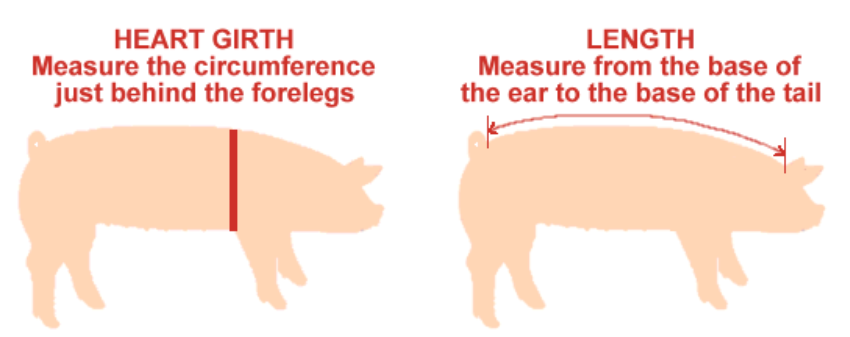
\includegraphics[height=0.25\textheight]{figures/Pig Tape Measure}
	\caption{Illustration of weight estimation using a tape measure}
	\label{fig:Tape Measure}
\end{figure}

\subsection{Modern Techniques}

Body weight (BW) prediction in livestock can be modeled using four main approaches of increasing complexity: Traditional Approach, Computer Vision Approach, Computer Vision with Machine Learning, and Computer Vision with Deep Learning. The Traditional Approach relies on manually collected morphometric measurements such as heart girth, wither height, and body length, which are then applied in traditional regression models. This method has been widely used for species such as cattle, pigs, sheep, goats, camels, and yaks \citep{franco2017evaluation}; \citep{fadlelmoula2020prediction}; \citep{yan2019body}. While effective, it is labor-intensive and causes stress to the animals. To mitigate these issues, the Computer Vision (CV) Approach uses 2D and 3D electro-optical sensors, such as RGB or Kinect cameras, to capture images for morphometric measurements \citep{ozkaya2013prediction}. Although 3D cameras improve precision, they are expensive and require complex data processing. The CV with Machine Learning (CV+ML) Approach enhances the CV method by automating feature selection with machine learning techniques, although some manual processes, such as image segmentation and morphometric extraction, remain necessary \citep{tasdemir2019ann}. Finally, the CV with Deep Learning (CV+DL) Approach uses deep learning models, including convolutional neural networks (CNNs) and recurrent convolutional networks (RCNNs), to fully automate the BW prediction process \citep{gjergji2020deep}. While this approach has shown significant improvements, challenges still exist in precisely segmenting animals from complex backgrounds \citep{shukla2016metric}. These approaches highlight the evolution of BW prediction models, transitioning from manual methods to fully automated systems, with deep learning offering promising advancements.

\subsection{Convolutional Neural Networks (CNN)}

Convolutional Neural Networks (CNNs) are a class of deep learning models specifically designed to process data with grid-like topologies, such as images. These networks employ a series of convolutional operations using trainable filters to detect local patterns (e.g., edges, textures, and shapes), which are then aggregated through pooling operations to reduce dimensionality while preserving essential information. At the final stages, fully connected layers interpret the abstracted features to generate predictions or classifications \citep{lecun2015deep_learning}.

What sets CNNs apart from traditional machine learning algorithms is their ability to automatically learn and optimize feature representations directly from raw pixel data, eliminating the need for handcrafted features and domain-specific input preprocessing. This makes them particularly suitable for complex image recognition and regression tasks where spatial hierarchies and relationships are crucial.

In the context of agriculture and livestock management, CNNs have been successfully deployed for various applications including species classification, posture detection, health monitoring, and behavioral analysis. One of the most promising applications of CNNs in this domain is livestock weight estimation, where non-invasive methods are favored over traditional weighing scales due to concerns about animal welfare, labor intensity, and logistical constraints.

Recent research has demonstrated the effectiveness of CNNs in predicting pig weight from overhead RGB images. For instance, \cite{pinto2024pig_weights} developed a CNN-based system that achieved a mean absolute percentage error (MAPE) as low as 1.35\%, even under varying lighting conditions and pig postures. This performance highlights CNNs' robustness in real-world environments, especially when paired with top-down image acquisition methods using cameras like the Microsoft Kinect. These models are trained to associate pixel-based spatial cues—such as body shape and area—with actual weight, achieving high accuracy without the need for manual measurements or handling.

Moreover, CNNs are well-suited for integration with depth image data, which is particularly beneficial in weight estimation tasks. Depth images add a third spatial dimension, enabling CNNs to interpret volume-related features more effectively. In the context of this study, the depth information captured using Kinect V1 enhances the CNN's capacity to infer body mass with greater precision by leveraging 3D structural information that 2D RGB images may not fully convey.

\subsection{CNN in Image Processing}

In the domain of image processing, Convolutional Neural Networks (CNNs) have become the foundational architecture for most modern computer vision applications. Their design, inspired by the visual cortex of animals, enables them to extract multiscale features by applying convolutional filters over local image regions. These features range from simple patterns like edges and corners in the early layers to more complex textures, shapes, and object structures in deeper layers \citep{krizhevsky2012imagenet}. This hierarchical feature extraction mechanism allows CNNs to perform exceptionally well on tasks such as image classification, segmentation, and object detection.

Unlike traditional image processing techniques that rely on handcrafted feature descriptors like SIFT or HOG, CNNs automatically learn relevant features from training data, which significantly improves accuracy and adaptability in diverse real-world scenarios. Their generalization capability has led to widespread use in industries ranging from healthcare and security to autonomous driving and agriculture.

In the context of livestock farming, CNNs have proven to be powerful tools for non-invasive visual analysis. They are commonly used for posture recognition, gait analysis, behavioral monitoring, and health condition assessment of animals. For example, CNN-based models have been applied to segment animals from backgrounds, detect body landmarks, and classify behavior patterns in cattle, poultry, and pigs \citep{andrasi2023pig_weight, wang2021deep_learning_farming}. This automation not only reduces the reliance on manual observation but also enables real-time monitoring, which is critical for early disease detection and animal welfare.

When paired with depth imaging technologies such as Microsoft Kinect, CNNs can process 3D spatial data, making them even more suitable for precision livestock applications. Depth images provide additional information about the spatial configuration and volume of animal bodies, which 2D RGB images alone cannot offer. CNNs trained on depth data can thus extract volumetric features essential for applications like weight estimation, where accurate assessment of body mass is required without direct contact.

Moreover, CNNs have been integrated into real-time farm monitoring systems, leveraging top-down camera views to continuously track animal growth. Studies have shown that CNNs can reliably identify individual pigs and estimate physical parameters such as body area and length, even in cluttered or low-contrast environments \citep{pinto2024pig_weights}. The use of depth maps enhances the segmentation and feature extraction process, particularly when lighting or posture varies, conditions commonly found in open or semi-controlled farm settings.

\subsection{Light Gradient Boosting Machine (LightGBM)}

Light Gradient Boosting Machine (LightGBM) is a highly efficient and scalable machine learning framework based on gradient boosting decision trees (GBDT). It was developed to overcome the computational limitations of traditional boosting algorithms, particularly when dealing with large-scale data and high-dimensional feature spaces. LightGBM adopts a novel leaf-wise tree growth strategy with depth limitations, which selects the leaf with the highest gain to grow, rather than the level-wise approach used in conventional GBDT models. This technique improves both the speed and accuracy of the model, while also effectively mitigating the risk of overfitting \citep{ke2017lightgbm}.

One of the defining advantages of LightGBM is its ability to handle large datasets with numerous features and missing values efficiently. It supports both categorical and continuous variables, and it performs well with skewed and sparse datasets—common conditions in agricultural image analysis where some features may dominate while others contribute noise.

In the context of animal agriculture, particularly for weight estimation tasks, LightGBM is often employed to analyze structured numerical data extracted from image or depth data. These features can include geometric measurements such as pixel size, volume proxy, standard deviation of depth, aspect ratio, and perimeter—all of which correlate with body mass. When combined with depth-sensing technology like the Microsoft Kinect V1, such features provide rich, non-contact input for predicting animal weight.

Recent studies have validated LightGBM’s effectiveness in livestock applications. For instance, in pig farming scenarios, features derived from top-view depth images—such as pixel count, mean depth, and shape ratios—were used as inputs to LightGBM regressors to estimate the live weight of pigs \citep{pezzuolo2018barn}. The models achieved high coefficients of determination (R²), often exceeding 0.95, indicating a strong correlation between image-derived features and actual body weight. Such results emphasize LightGBM's capability to model nonlinear relationships inherent in biological data.


\subsection{Applications of Kinect in Agriculture}

In livestock farming, Kinect sensors are used to monitor animal behavior, health, and growth through 3D imaging. This technology allows for early detection of health issues by analyzing subtle changes in posture, gait, and movement patterns. It can identify lameness in cattle early on, allowing for prompt intervention \citep{singh2022smart}. Moreover, Kinect’s non-invasive methods provide automated weight estimation by capturing 3D images, reducing the need for stressful manual weighing processes. Continuous monitoring helps track growth and optimize feeding schedules, contributing to the overall welfare of livestock. In addition to health monitoring, Kinect sensors contribute to environmental control within livestock facilities, tracking variables like temperature and humidity to ensure optimal conditions. In poultry farming, Kinect can monitor flock movement patterns, alerting farmers to potential issues like overcrowding, which could lead to health or productivity problems.

The integration of Kinect into Precision Livestock Farming (PLF) systems further enhances its value, as it collects real-time data alongside other technologies like RFID and GPS. This combination allows for more efficient resource management, improved reproductive tracking, and more precise feeding practices \citep{monteiro2021precision}. Kinect technology is also being used in crop management. Its 3D imaging capabilities are beneficial in monitoring plant growth, detecting diseases early, and optimizing resource use like water and fertilizers. In automated harvesting, Kinect sensors guide robots through fields, identifying ripe crops based on their size and shape. This reduces the need for manual labor and ensures timely harvesting to maximize yield and quality \citep{singh2022smart}.

\section{Microsoft Kinect V1}

The Kinect V1 sensor employs an infrared (IR) structured light system to capture depth information. It consists of three main components: an RGB camera, an IR projector, and an IR sensor. The RGB camera captures standard color images, while the IR projector emits a structured pattern of infrared light onto the environment. The IR sensor detects distortions in the projected pattern caused by objects in the scene, enabling the device to compute depth information based on the time and spatial displacement of the reflected IR light \citep{Zhang2012}. This technique provides a depth resolution of 640x480 pixels, with a frame rate of up to 30 frames per second, making it suitable for capturing detailed spatial data.

\subsection{Depth Data Acquisition and Processing}

The Kinect V1 produces a 3D point cloud by combining depth and RGB data, representing the spatial coordinates (X, Y, Z) of each pixel in the captured scene. This depth information is particularly useful for applications requiring precise measurements of object size, shape, and volume. The sensor's effective depth range is between 0.8 and 4.0 meters, allowing it to capture accurate data within typical livestock pen dimensions \citep{Smisek2013}. By leveraging its depth-sensing capability, researchers can measure the dimensions of objects without physical contact, making it ideal for non-invasive weight estimation in pigs.

\subsection{Kinect V1 Applications in Agriculture}

The Kinect V1 has been successfully utilized in agricultural studies for tasks such as plant phenotyping, fruit grading, and livestock monitoring. For instance, \citep{Andujar2016} used the Kinect V1 to evaluate crop height and canopy structure, demonstrating its utility in capturing detailed morphological data. Similarly, \citep{pezzuolo2018barn} employed the Kinect V1 to estimate cattle body volume and weight, achieving high accuracy compared to traditional methods. These applications highlight the potential of the Kinect V1 as a versatile tool for precision agriculture.

\subsection{Kinect V1 Potential for Pig Weight Estimation}

In pig farming, accurate weight estimation is crucial for optimizing feeding strategies and monitoring growth. Traditional weighing methods, such as scales or manual measurements, can be labor-intensive, stressful for animals, and prone to errors \citep{faucitano2018transport}. The Kinect V1 offers a non-invasive alternative by capturing detailed depth images that enable the calculation of pig body volume. By processing these depth images using machine learning algorithms, it is possible to develop a system that estimates pig weight based on 3D body volume, eliminating the need for physical contact.

The Kinect V1's structured light technology ensures that depth measurements are unaffected by variations in visible light conditions, making it suitable for use in indoor pig pens where lighting may vary. Additionally, its ability to provide real-time depth data opens the possibility for developing dynamic weight monitoring systems that can track pig growth continuously.


\section{Synthesis Matrix}

The synthesis matrix provides valuable insights into pig weight estimation methods using various imaging and analysis techniques. Together, these studies provide a cohesive foundation for applying Kinect technology, advanced imaging, and regression methods in the current study, demonstrating approaches for accurate, adaptable, and practical pig weight estimation.
\newpage
\begin{longtable}{|p{0.15\linewidth} | p{0.15\linewidth} | p{0.2\linewidth} | p{0.2\linewidth} | p{0.15\linewidth}|}
	\caption{Synthesis Matrix}
	\label{tab:synthesis matrix}\\
	\hline
	\textbf{Title} & \textbf{Author(s), Year} & \textbf{Methodology} & \textbf{Findings} & \textbf{Relevance} \\
	\hline
	On-barn pig weight estimation based on body measurements by a Kinect v1 depth camera
	& 
	Pezzuolo, A., Guarino, M., Sartori, L., González, L. A., and Marinello, F. (2018) 
	&
	- Kinect v1 Depth Camera\newline
	- Estimated pig weight from body measurements\newline
	- Captured 3D images in a barn environment\newline
	- Extracted length, width, and volume from depth data\newline
	- Developed a regression model for weight estimation
	& 
	Both linear and second-degree regression models showed strong correlations with reference weights, with coefficients of determination above 0.95. The non-linear model reduced the standard error by half, and the second-degree regression model had an absolute error of less than 0.5 kg.
	&
	The current study is closely correlated with this study, especially in terms of the usage of the Kinect v1 camera. This study, however, uses 3D images for the calculation of estimated weights.
	\\
	\hline
	Pig Weight Estimation According to RGB Image Analysis
	& 
	Andras Kárpinszky, Gergely Dobsinszki(2023)
	&
	- RGB Cameras (Dahua Models)\newline
	- RGB image captured above pig pens\newline
	- Mask R-CNN for segmentation\newline
	- Kalman filters for tracking\newline
	- Pretty Contour Picker (PCP) for filtering\newline
	- Weight estimation using Multi-Layer Perceptron (MLP)
	& 
	The system achieved more than 97 percent accuracy in predicting pig weights compared to manually recorded weights. Among the models tested, Model V2 was the most consistent, providing high accuracy across varying weight ranges. The RGB image-based method allows faster and stress-free weight measurement, which is valuable for decision-making in pig farming
	&
	Although a Kinect camera wasn’t used in the study, the setup for data acquisition and processing is similar. Top-view photos of pigs were also used in this study, closely relating to how the current study takes them.
	\\
	\hline
	Estimating Pig Weights from Images without Constraint on Posture and Illumination
	& 
	Kyungkoo Jun, Si Jung Kim, Hyun Wook Ji (2018)
	&
	- 2D Image Processing\newline
	- No relaxed posture and illumination constraints\newline
	- Image processing: binarization, morphological ops, contour analysis\newline
	- Features: area size, curvature, deviation\newline
	- Neural network model trained and tested for weight prediction
	& 
	The study achieved an average estimation error of 3.15 kg and a coefficient of determination (R²) of 0.792. Despite this being lower than previous works, the method was able to estimate pig weights without controlling the environment, posture, or lighting, making it applicable in less constrained settings. The model showed that posture-related features contributed significantly to weight prediction accuracy.
	&
	The study utilized a 2D camera, meanwhile the current study will utilize a Kinect v1 camera. Despite the difference, both studies have similar top-down view camera setups. The idea of estimating pig weights without constraints on posture and illumination can also be an inspiration for future similar undertakings with the Kinect v1 camera.
	\\
	\hline
	Carcass Quality Traits of Fattening Pigs Estimated Using 3D Image Technology
	& 
	A. Peña Fernández, T. Norton, E. Vranken, D. Berckmans (2019)
	&
	- Kinect 3D Cameras\newline
	- Capture 3D top-view images pre-slaughter.\newline
	- Extract image features: lengths, areas, and volumes.\newline
	- MATLAB for stepwise linear regression analysis
	& 
	The regression models achieved an adjusted R² ranging from 70-85 percent during training, but performance decreased to 50-60 percent during validation. The best correlations with slaughter traits, such as final weight and yield, were found using the median values of image features from the last week of the fattening period.
	&
	Considering only the sections relevant to pig weight estimation, the study can be used as a reference for the current study given that it also uses Kinect cameras for image capture. The methods for feature extraction and pig weight estimation and analysis can be used as one of the bases for the methods that will be used in the current study.
	\\
	\hline
\end{longtable}

The synthesis matrix provides valuable insights into pig weight estimation methods using various imaging and analysis techniques. The first study by \citep{pezzuolo2018barn} effectively demonstrates using a Kinect v1 depth camera to capture 3D body measurements, achieving high prediction accuracy with regression models, particularly a second-degree regression model that reduced error to under 0.5 kg. This finding supports the current study’s use of Kinect v1 for accurate weight estimation via 3D imaging. 

In another study, \citep{karpinszky2023pig} employed RGB cameras combined with segmentation (Mask R-CNN) and MLP models, achieving over 97 percent accuracy in weight prediction. Although RGB cameras differ from Kinect, the segmentation and tracking methods align well with the current study’s top-view imaging approach and offer potential techniques for data processing in the project.

The work of \citep{jun2018estimating} further broadens applicability by achieving weight estimation without controlling for pig posture or lighting, using a neural network model on 2D images with a 3.15 kg error margin. This flexibility offers useful insights into handling environmental variability, which could enhance the robustness of your Kinect-based approach. 

Lastly, \citep{pena2019carcass} applied Kinect-based 3D imaging for carcass trait prediction, with results showing time-evolving feature accuracy between 50-85 percent. Their regression techniques could be useful for refining the project’s model to predict weight accurately.
Together, these studies provide a cohesive foundation for applying Kinect technology, advanced imaging, and regression methods in the current study, demonstrating approaches for accurate, adaptable, and practical pig weight estimation.

}